% !TeX root = ../main.tex
% LLD: Low Level Design

\chapter{详细设计与实现}

本章节主要在概要设计的基础之上,对本中文时间表达式信息抽取系统的详细设计给出具体解决方案并进行实现,其内容主要包括各个模块的详细设计和逻辑实现。
本章节深入理解概率无关上下文语法的原理及其工作的上下文环境,设计实现各种识别和解析规则,完成本中文时间表达式信息抽取系统的编码实现。

\section{中文时间表达式识别模块的设计与实现}

\subsection{概述}

中文时间表达式的识别和解析都是以概率无关上下文语法为核心算法实现的。
对于中文时间表达式,涉及到两个比较关键的部分,一部分是对数字部分的识别,另一部分是对时间单元的识别,最后是有机的将这些识别规则组合到一起。
概率无关上下文语法通常四元组的形式出现: (N,R,S, $\varSigma$)。 其中N代表的是非终止符号集合,$\varSigma$ 代表的是终止符号的集合,$\varSigma$。
R代表的是一规则或者是产生式的结合,对于每一个产生式,其组成形式应该为 A $\rightarrow$ $\beta$[p],其中A应该为一个非终止符,beta是一个包含0个或多个符号的字符串,
字符串的形式应该为($\varSigma$ $\cup$ N),即非终结符与终结符的交集中产生的字符串。 p则为一个介于0和1中间的数字,表示 P($\beta$|A)的概率。
P($\beta$|A)可以理解为由终止符产生相应的表达式字符串的概率,即该产生式的概率。
S则为起始符号。


\subsection{数值类型识别子模块的设计与实现}

\subsubsection{数值类型终止符定义的设计与实现}

\begin{table}[h]
    \centering
    \caption{部分数值类型终止符}
    \begin{tabular}{*{4}{c}}
        \toprule
        类名                  & 描述                            & 蕴含字符                       & 对应数字                          \\
        \midrule
        CHINESE\_DIGITS       & 简体中文数字                    & \makecell*[c]{〇,一,二,三,四,                                    \\ 五,六,七,八,九} & \makecell*[c]{0,1,2,3,4,\\ 5,6,7,8,9}         \\
        CHINESE\_DIGITS\_TRAD & 繁体中文数字                    & \makecell*[c]{零,壹,贰,叁,肆,                                     \\ 伍,陆,柒,捌,玖}  & \makecell*[c]{0,1,2,3,4,\\ 5,6,7,8,9}         \\
        CHINESE\_UNITS        & \makecell*[c]{简体中文数字单位} & \makecell*[c]{十,百,千,                                         \\ 万,十万,百万}     & \makecell*[c]{$10^1,10^2,10^3,$ \\ $10^4,10^5,10^6$} \\
        CHINESE\_UNITS\_TRAD  & \makecell*[c]{繁体中文数字单位} & 拾,佰,仟,萬,億                 & \makecell*[c]{$10^1,10^2,10^3,$ \\ $10^4,10^8$}       \\
        ARABIC\_DIGIT         & 阿拉伯数字                      & \makecell*[c]{0,1,2,3,4,                                      \\ 5,6,7,8,9} & \makecell*[c]{0,1,2,3,4,\\ 5,6,7,8,9}         \\
        MIXED\_SIGNS          & 正负符号                        & 正,+,负,-                   & 1,1,-1,-1                      \\
        \bottomrule
    \end{tabular}
    \label{tab:numeral_terminal}
\end{table}

数值类型终止符主要涉及到阿拉伯数字与中文数字的识别,出于使用场景的考虑,文字识别中并没有带上英文数字表示,那已经超过日常生产环境的使用范围。

数值类型终止符主要通过继承TerminalSymbol类实现。 每一个继承该类的子类都为相应的终止符。 数值类型中比较核心的类有Comma,ArabicDigit,MixedSign,ChineseDigit,ChineseUnits。
数值类型终止符相关类的类图可见图~\ref{fig:numeral_terminal}。
如图中所示,每个终止符类中都包含一个RECOGNIZER字段,该字段对应RegexRecognizer类,此类为正则表达式的正则表达式解析器,可以将终止符定义的文字符号组织成正则表达式规则以解析我们需要处理的自然语言文本。
以ArabicDigit类为例,其对应的文字符号将通过RegexRecognizer类的generate\_terminals方法组织成为 '$\left[ 0123456789 \right]$'的正则表达式形式,并通过Python语言底层的re模块,即正则表达式解析模块实例化为正则表达式类。
每个类对应的具体的自然语言文本可见表~\ref{tab:numeral_terminal}。


\begin{figure}[h]
    \centering
    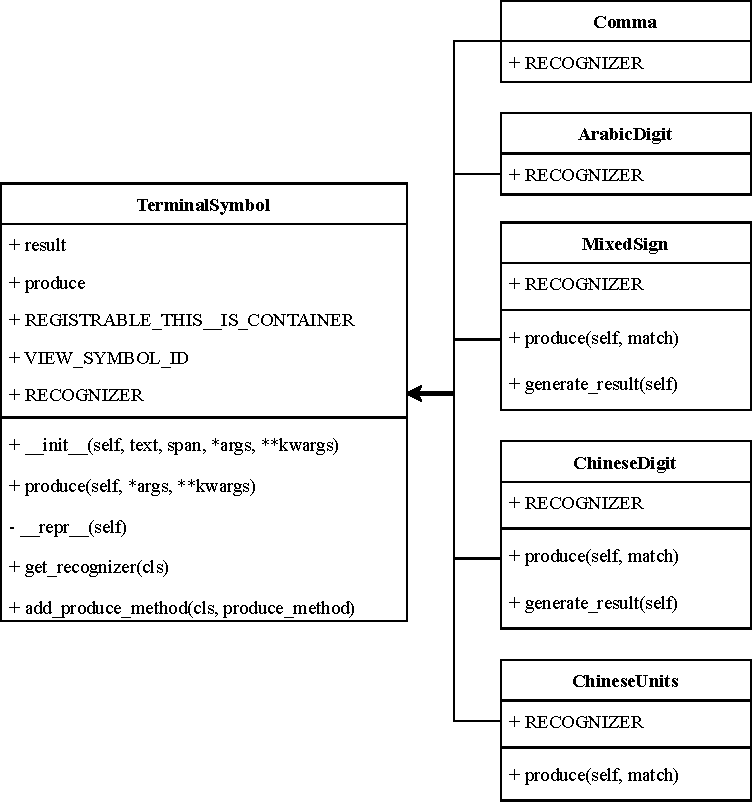
\includegraphics[width=0.8\textwidth]{numeral_terminal.pdf}
    \caption{数值类型终止符号类图}
    \label{fig:numeral_terminal}
\end{figure}


\subsubsection{数值类型非终止符的设计与实现}

数值类型非终止符的主要实现类需要继承NonTerminalSymbol,如图~\ref{fig:numeral_nonterminal}所示。
列举出来的一些NonTerminalSymbol的子类包括ChineseMixedDigitsAndUnits,MixedChineseArabicDigits,ArabicDigits,ChineseArabicDigit,MixedDigitOom等整数类型。
浮点数,百分数等类就不一一列举出来。 每个继承类的内部会包含RULE字段,该字段主要作用在于方便在解析的过程中收集与之相关的产生式。 部分数值类型非终止符的产生式如表~\ref{tab:numeral_nonterminal}。

数值类型非终止符起到的作用是集合或生成终止符或其他非终止符,和一般性的上下文无关语法不同,在中文时间表达式识别过程中,所有能够匹配给定文本中某一部分的规则,
其所匹配到的信息都具有一定的价值,所以在组合规则的过程中,会自然的形成类似于抽象语法树的结构,会在树中结点贮存相关的文本信息。
因为此原因,每个继承NonTerminalSymbol的子类都需要显示的指定其是否为最终的起始符号,也就意味着,最终产生的概率无关上下文语法中,将会有一个或多个起始符号,可以根据IS\_GOAL字段是否为真进行判断。
并在后续过程中通过VIEW\_SYMBOL\_ID字段进行收集,再根据其实符号的概率值进行判断排序并输出结果。

为了和非终止符,也就是TerminalSymbol类做出区分。
NonTerminalSymbol中存在REGISTRABLE\_THIS\_IS\_CONTAINER字段,
将继承非终止符类的子类作为容器,装载一个或者多个产生式,不同的产生式将会按照
produce\_index\_in\_rule的形式,由专门的python元类处理,表示不同的产生式。 如表~\ref{tab:numeral_nonterminal}中的MixedChineseArabicDigits类,因其关联到两个不同的产生式,所以其将分别
注入 produce\_0$\left(self,mixed\_digits,chinese\_units\right)$和produce\_1$\left(self,arabic\_unsigned\_integer,chinese\_units\right)$两个方法,方法中的参数为对应的产生式右侧的终止符或者非终止符。


\begin{table}[h]
    \centering
    \caption{部分数值类型非终止符及产生式}
    \begin{tabular}{*{4}{c}}
        \toprule
        类名 & 描述 & 部分产生式示例 & 文本示例 \\
        \midrule
        \makecell*[c]{CHINESE\_
            \\ MIXED\_DIGITS \\ \_AND\_UNITS} & \makecell*[c]{中文阿拉伯\\数字混合类型} & \makecell*[c]{\textit{SelfRefSymbol}  \rightarrow \\ MixedDigits + ChineseUnits;
            \\ \textit{SelfRefSymbol} \rightarrow \\ ArabicUnsignedInteger + ChineseUnits} & \makecell*[c]{3千4百\\八十六万} \\
        \makecell*[c]{ARABIC\_                  \\ DIGITS}    & \makecell*[c]{阿拉伯数字} & \makecell*[c]{\textit{SelfRefSymbol}   \rightarrow
            \\ SelfRefSymbol + ArabicDigit; \\  \textit{A}   \rightarrow \\  ArabicDigit   }  & 123045 \\
        \makecell*[c]{MIXED\_                   \\ DIGIT\_OOM} & \makecell*[c]{混合型数字} & \makecell*[c]{\textit{SelfRefSymbol}   \rightarrow
            \\ MixedChineseArabicDigits + ChineseDigits; \\  \textit{SelfRefSymbol}   \rightarrow \\  MixedArabicChineseDigits + ArabicUnsignedInteger;
            \\  \textit{SelfRefSymbol} \rightarrow \\ MixedChineseArabicDigits + ArabicUnsignedInteger;
            \\   \textit{SelfRefSymbol} \rightarrow  MixedChineseArabicDigits;
            \\   \textit{SelfRefSymbol} \rightarrow  MixedArabicChineseDigits;
            \\ \textit{SelfRefSymbol} \rightarrow  ChineseDigits }  & \makecell*[c]{1二3\\四567} \\
        \bottomrule
    \end{tabular}
    \label{tab:numeral_nonterminal}
\end{table}

\begin{figure}[h]
    \centering
    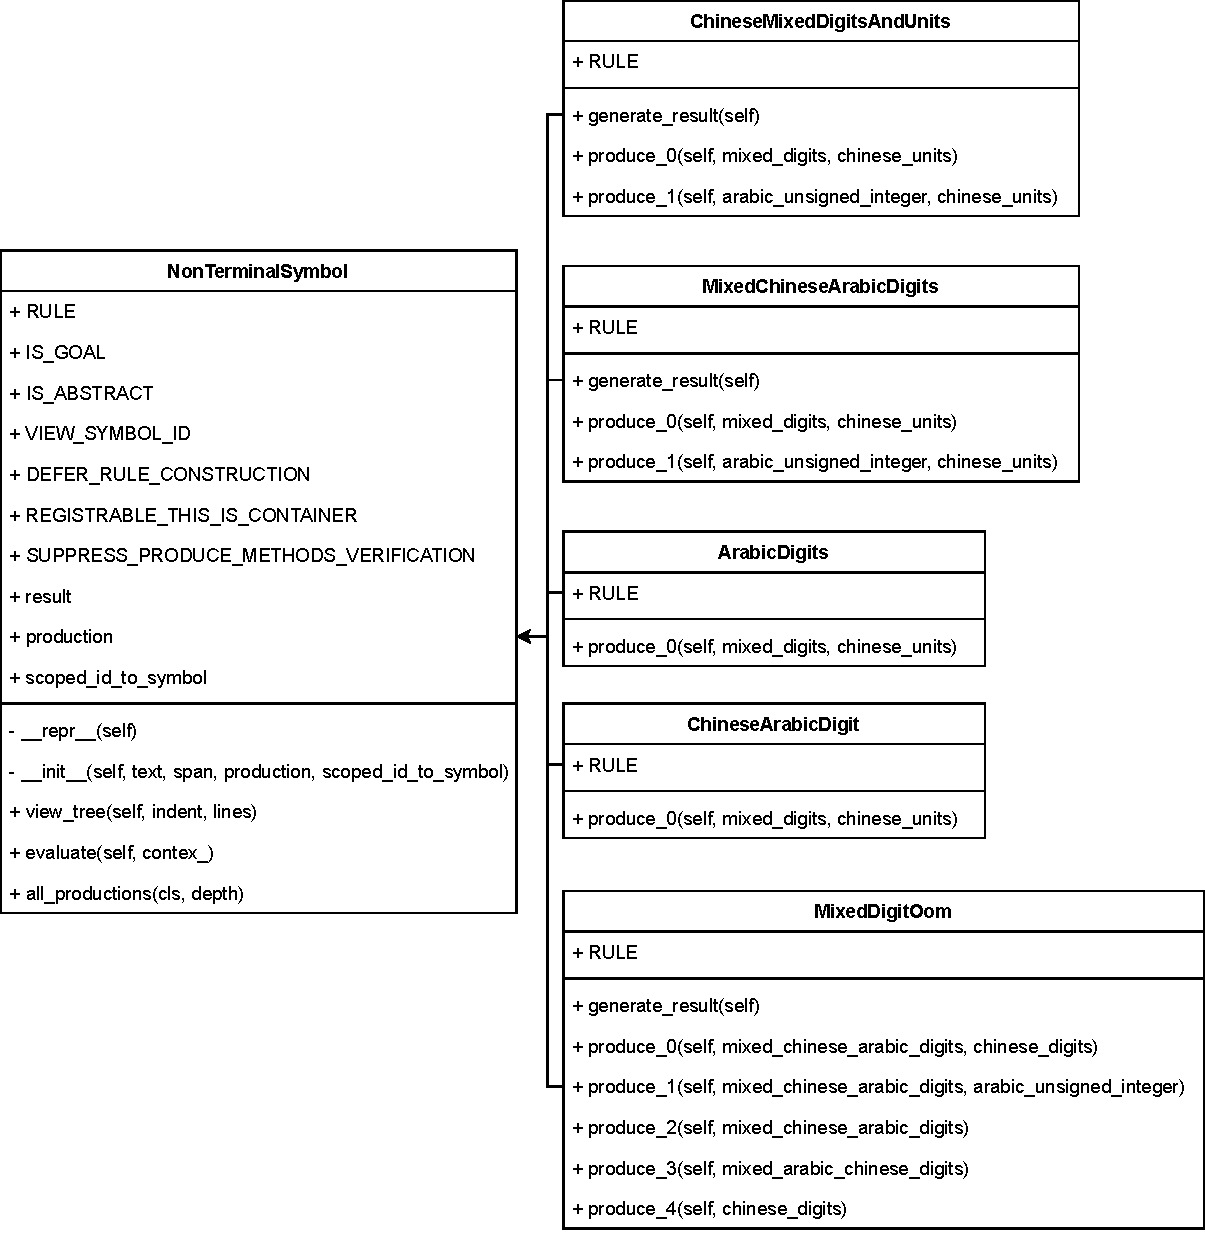
\includegraphics[width=1\textwidth]{numeral_nonterminal.pdf}
    \caption{部分数值类型非终止符号类图}
    \label{fig:numeral_nonterminal}
\end{figure}

\subsection{时间单元识别子模块的设计与实现}

\subsubsection{时间单元终止符的设计与实现}

时间单元终止符的设计主要考虑到中文时间表达的多个时间维度即修饰符,包括但不限于:
\begin{enumerate}
    \item 时间刻度,如1998年,9月18日下午两点,周六晚七点等;
    \item 时间段,如三天,24小时,一个钟头等;
    \item 时间方位词,如前,后,去,下等;
    \item 量词,如个,半等;
    \item 特殊事件,如中秋节,国庆,辛亥革命。
\end{enumerate}

考虑到上述情况,针对不同的时间维度,时间范围和相应的修饰符,表~\ref{tab:date_terminal}列举出部分时间单元终止符及其描述。

\begin{table}[h]
    \centering
    \caption{部分时间单元终止符}
    \begin{tabular}{*{4}{c}}
        \toprule
        类名            & 描述                 & 蕴含字符                                 \\
        \midrule
        DUR\_UNIT\_HOUR & 以小时为单位的时间段 & 小时                                     \\
        QUANTIFER       & 量词                 & 个                                       \\
        UNIT\_WEEK      & 以周为单位的时间刻度 & $\left(\text{周|星期|礼拜}\right)$       \\
        UNIT\_THIS\_ADV & 副词,表示当前状态   & $\left(\text{这|今|本}\right)$           \\
        EVENT           & 特殊事件             & $\left(\text{中秋|国庆|星海革命}\right)$ \\
        \bottomrule
    \end{tabular}
    \label{tab:date_terminal}
\end{table}


时间单元终止符的实现与数值类型终止符的实现大同小异,都需要继承TerminalSymbol类。 其部分类图如~\ref{fig:date_terminal}所示。
其中比较典型的类有DurUnitHour,Quantifier,UnitWeek,UnitThisAdv,Event。


\begin{figure}[h]
    \centering
    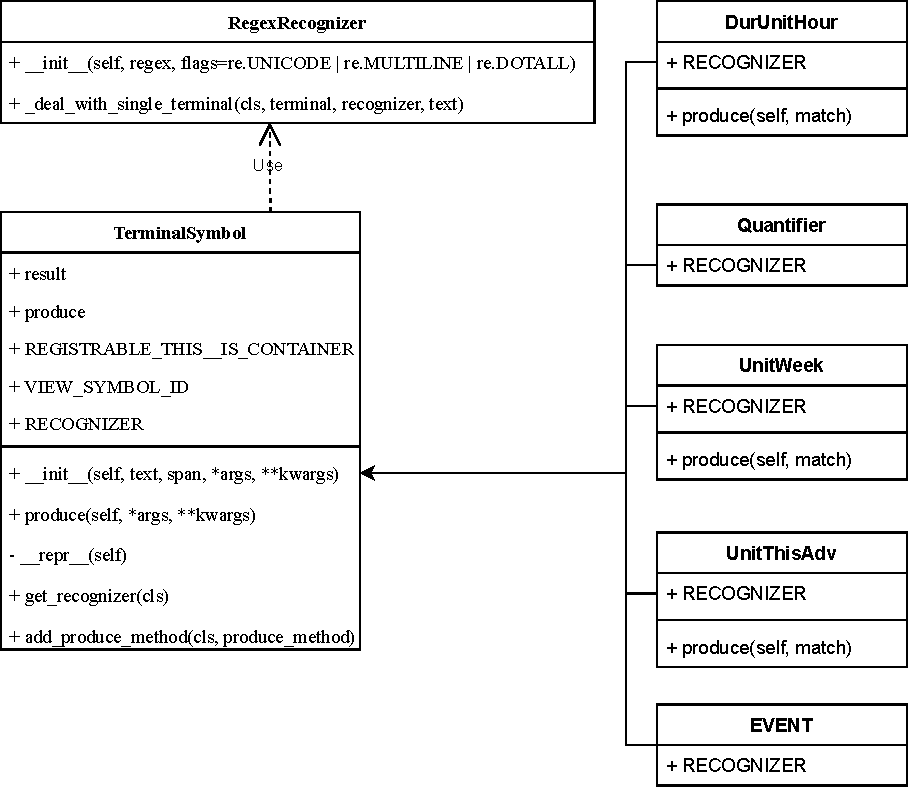
\includegraphics[width=0.75\textwidth]{date_terminal.pdf}
    \caption{部分时间单元终止符号类图}
    \label{fig:date_terminal}
\end{figure}

\begin{figure}[h]
    \centering
    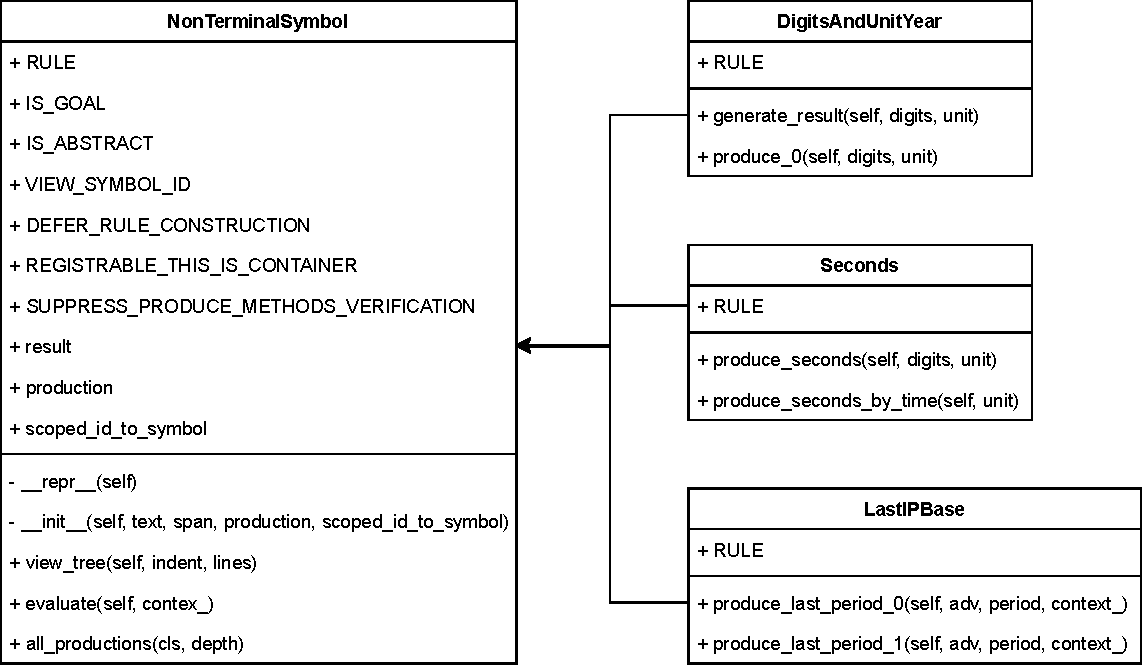
\includegraphics[width=1\textwidth]{date_nonterminal.pdf}
    \caption{部分时间单元非终止符号类图}
    \label{fig:date_nonterminal}
\end{figure}


\subsubsection{时间单元非终止符的设计与实现}


实现时间单元非终止符的具体实现类除了要继承NonTerminalSymbol类,还需要依赖与数值类型的终止符与非终止符。 部分实现类如下图~\ref{fig:date_nonterminal}所示。
时间单元非终止符的设计方式与时间单元终止符的设计思路保持一致,同样按照中文时间表达的多个时间维度(如小时,年月日等),时间范围(一段时间),关于时间的修饰符等进行规则设计和实现。


\section{中文时间表达式解析模块的设计与实现}

\begin{figure}[h]
    \centering
    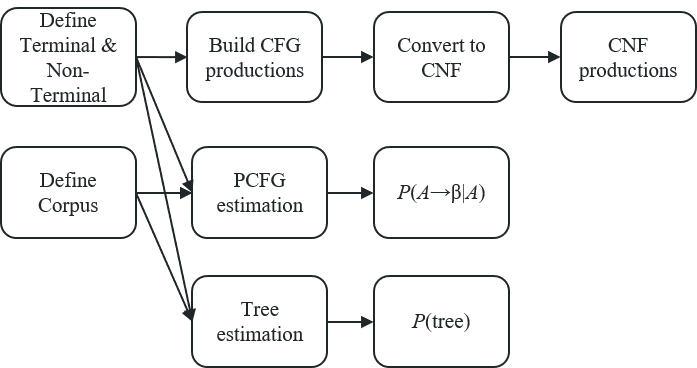
\includegraphics[width=0.7\textwidth]{preprocess.pdf}
    \caption{预处理过程示意图}
    \label{fig:preprocess}
\end{figure}


\subsection{预处理过程的设计与实现}

在前文中已经给出定义与时间表达式相关的终结符(terminal)和非终结符(non-terminals),终结
符在文本匹配中类似于正则表达式,以确定时间表达式的区间(span)。非终结符则在最后对
时间表达式抽象成的语法树中充当非叶结点。图~\ref{fig:preprocess}中由终结符和非终结符组成的产生式
(production)最终将被简化为 CNF(Chomsky norm function)。同时我们需要向语料库中写入
语料,语料库中的每条数据应该以(文本,结果)的文本对的形式存储,语料库作为训练集以
求得每个产生式的似然。产生式的似然将参与求得语法树整体概率的计算。

\subsection{分析树的构建过程的设计与实现}

\begin{figure}[h]
    \centering
    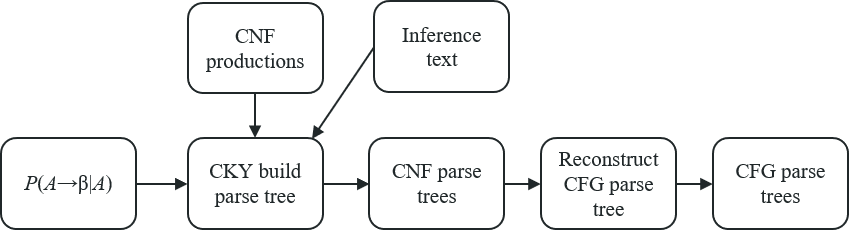
\includegraphics[width=1\textwidth]{tree_construction.pdf}
    \caption{分析树的构建过程示意图}
    \label{fig:tree_construction}
\end{figure}

分析树的构建过程如图~\ref{fig:tree_construction}所示,在获取产生式的似然和简化CFG产生式为CNF后,我们输入需要推理的文本(inference text),以识别文本中的时间表达式,并为识别出的时间表达式构建语法分析树。
同一时间表达式可能存在不同的解析方式,即不同的解析树,我们利用产生式的似然与CKY算法(Cocke–Younger–Kasami algorithm)推导最终可能产生的零个或多个CNF解析树。分析树构建过程可见算法~\ref{algo:tree_construction}
随后我们将CNF解析树还原为CFG解析树,以还原分析树的初始状态。此时,解析树中的非叶结点为上一小节中的非终结符,叶结点为终结符。图~\ref{algo:tree_construction}举例了一个时间表达式可能被解析成的一棵语法树。
左边分析树识别时间段(period),三日(3 days),右边分析树识别日期(date)十月三日(October 3rd),识别区间存在交集。 分析树构建过程中,会调用树中各个结点的get\_result方法,将结点作为可加和性质的元素进行计算。 图
图~\ref{fig:tree_construction}中结点所含有的值即为分析树构建过程中的计算结果。


\begin{figure}[h]
    \centering
    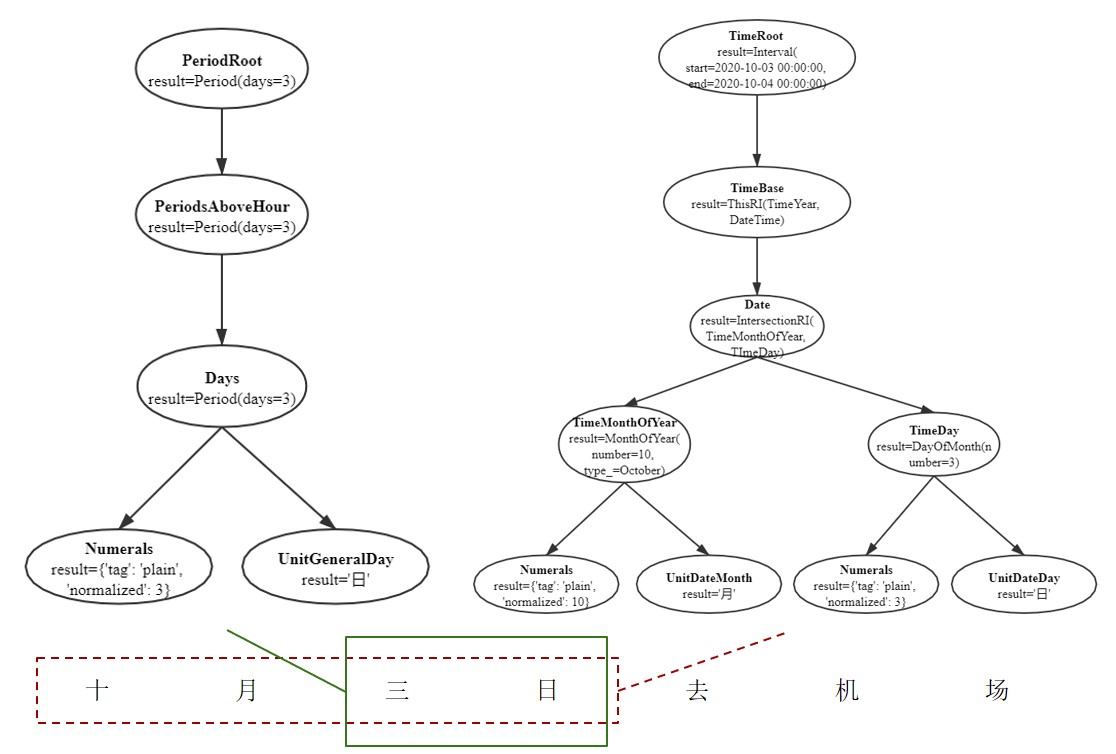
\includegraphics[width=1\textwidth]{example_1.pdf}
    \caption{时间表达式的语法冲突}
    \label{fig:example_1}
\end{figure}

\begin{algorithm}[h]
    \SetAlgoLined
    \KwData{分析树构建算法}
    \KwResult{具有最大概率的一棵树以及该树的概率 }
    initialization\;
    \For{$j=0$; $j<length of input$; $j++$} {
        \ForAll{$A | A \rightarrow input[j] \in grammar$}{
            table[j - 1,j,A] \leftarrow P(A \rightarrow input[j])
        }
        \For{$i=j-2$; $i\ge0$; $i--$}{
            \For{$k=i+1$; $k<j$; $k++$}{
                \ForAll{$A | A \rightarrow BC \in grammar$ {\bf and} $table[i,k,B] \ge 0$ {\bf and} $table[k,j,c] \ge 0$}{
                    \If{table[i,j,A] \less P(A \rightarrow BC) \times table[i,k,B] \times table[k,j,c]}{
                        table[i,j,A] \leftarrow  P(A \rightarrow BC) \times table[i,k,B] \times table[k,j,c] \\
                        back[i,j,A] \rightarrow {k,B,C}
                    }
                }
            }
        }
    }
    \caption{分析树构建算法}
    \label{algo:tree_construction}
\end{algorithm}


\subsection{冲突消解的设计与实现}


\begin{figure}[h]
    \centering
    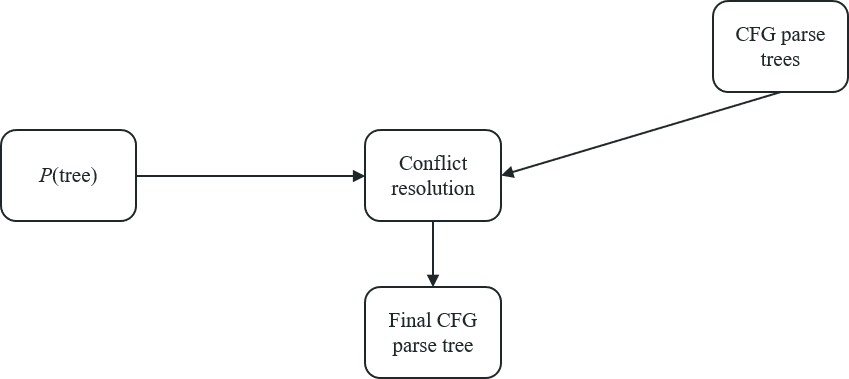
\includegraphics[width=0.8\textwidth]{conflict_resolution.pdf}
    \caption{冲突消解过程示意图}
    \label{fig:conflict_resolution}
\end{figure}

如图~\ref{fig:conflict_resolution},同一个时间表达式可能解析出多棵语法树,需要最终选择在总概率上为 top-k 的
k 棵语法树,即总体概率最大的 k 棵树。解析树的整体概率为树上所有产生式概率的乘积,则最终的语法树的概率如下。S 表示识别到的时间表达式,Tree 为
生成的解析树,n 为树中产生式的数量。




\subsection{中文时间表达式的归一化}

在使用句法分析获得时间表达式的语法树后,我们还需要将整棵树归一化到一种具体的
标注格式,这里我们选择了 SCATE 并加以改良,使其更贴合与中文的时间表达。归一化核心
的数据结构有三:
\begin{enumerate}
    \item Period:时间轴上的基本时间单位数量之和,如‘3 天’,‘2 个小时 30 分钟’;
    \item Interval:时间轴上一段左闭右开的,能确定到年份(year)的区间,如‘2019 年’,‘2019 年 3 月’;
    \item Repeat-interval:时间轴上一段左闭右开的,不包括年份,表示在时间轴上具有重复性的一段区间,如‘3 月份’,‘5 点 20 分’。
\end{enumerate}

我们以三种数据结构为核心,并用操作符集合(operator set)来表示时间表达式的语义,操作符本身也会继承NonTerminal类,并且作为分析树的根节点汇集树中所有结点的信息。
在表~\ref{tab:operator} 中列举出部分典型操作符,其中RI,I,P分别为Repeat-interval,Interval,Period的缩写。在构建时间表达式分析树的过程中,其实已经将操作符与数
据结构相结合,分析树构建完成后,树的根结点会将操作符集合形成嵌套表达式保存,直到我
们需要将时间表达式转化为特定的结构化信息时,才进行嵌套表达式的计算,以实现惰性计算
(lazy evaluation)。根结点的最终计算结果应该是以 ISO 格式描述的有起止时间的区间或类似
格式的时间段,如‘2019 年 3 月 2 日’,表达式最终计算的结果应该为‘Interval(start=2019-03-
02T00:00:00,end=2019-03-03T00:00:00)’。


\begin{table}[h]
    \centering
    \caption{部分操作符语义}
    \begin{tabular}{*{4}{c}}
        \toprule
        操作符         & 函数                                  & 描述                                    & 文本示例     \\
        \midrule
        SumP           & SumP(P,P) \rightarrow P              & 两个Period之和                          & 两小时20分钟 \\
        IntersectionRI & \makecell*[c]{IntersectionRI(RI,RI) \\ \rightarrow RI} & \makecell*[c]{两个Repeat-Interval\\ 之间的交集}           & 8月十五日    \\
        ThisRI         & ThisRI(I,RI) \rightarrow  I          & \makecell*[c]{根据Repeat-Interval\\确定年份}             & 8月十五日    \\
        BeforeIP       & BeforeIP(I,P) \rightarrow  I         & \makecell*[c]{将Interval向前\\移动Period的时间长度 }     & 三天前       \\
        AfterRI        & AfterRI(I,RI) \rightarrow  I         & \makecell*[c]{重新定位Repeat-Interval \\ 在时间轴上的区间} & 3月25日以后  \\
        \bottomrule
    \end{tabular}
    \label{tab:operator}
\end{table}




\section{时间信息抽取系统分析与展示模块}


对于训练好的中文时间表达式信息抽取系统,本地测试达到精度要求后,需要上线让用户使用,此时需要提供接口调用模型,企业内部对于用户提供了两种服务方式:SaaS 平台服务和线上 web 使用服务。

\subsection{SaaS服务}

SaaS 服务应用于整个智能文档处理平台,综合了 OCR 识别,语料抽取,实体识别,中文时间表达式信息抽取和其他模型等,旨在让用户根据需求选择对应服务。SaaS 平台服务可以方便地实现模型的参数更新,还可以给用户更多的选择空间,用户不仅可以
上传和标注训练数据以更新模型参数并进行测试,还可以利用 微调选项 单独训练自己的特殊样本。在整个 SaaS 服务平台中,用户上传文档后通过 OCR 或直接文本读取进行
字符提取,然后使用模型识别表格结构以及分析表格关系,同时结合 UI 界面让
用户方便地得到所需结果,极大地提高用户体验。

\subsection{web服务}

Web 服务旨在通过网络请求获取结果,此时用户上传文件并调用接口发送请
求,之后服务器接收数据进行文本预测,再返回用户需要的结果。对于 web 配置
使用公司内部自研的模块化的工作平台Metis。
Metis 指的是将模块组装成机器人并运行的平台,module 指 metis 平台上的
模块,是机器人组成的最小单元,机器人(dag)是将 module 按照一定的执行流
组装后的有向无环图,本质上是一个有向无环图的执行流,worker 指运行一组特
定组下的 module 环境,group 代表 module 可以从属于某些组。
机器人工作的流程为:

\begin{enumerate}
    \item 组装好机器人,按下启动键
    \item metis-mt 获取机器人的信息(dag),找到当下要执行的 module
    \item metis-mt 向任务池发送了一条这个 module 运行的请求,包含这个 module的 inputs、outputs、options 等,其中 inputs、outputs 的值是一段 short-id,指向真实数据的地址
    \item 相应的 worker(每个 worker 都知道自己能运行哪些 module,只有自己的他们才会拿来做)从池子中认领到任务
    \item 解析输入,将输入从一个地址信息转换为真实的内存数据,通过 module的定义来调用
    \item Module 开始进行处理
    \item Module 处理完了之后,将结果以元组的形式传回去
    \item Worker 将数据反序列化并按照请求放到指定地点
    \item 返回给 metis-mt,告诉他执行结果
    \item 重复执行 2-9
\end{enumerate}


\begin{figure}[h]
    \centering
    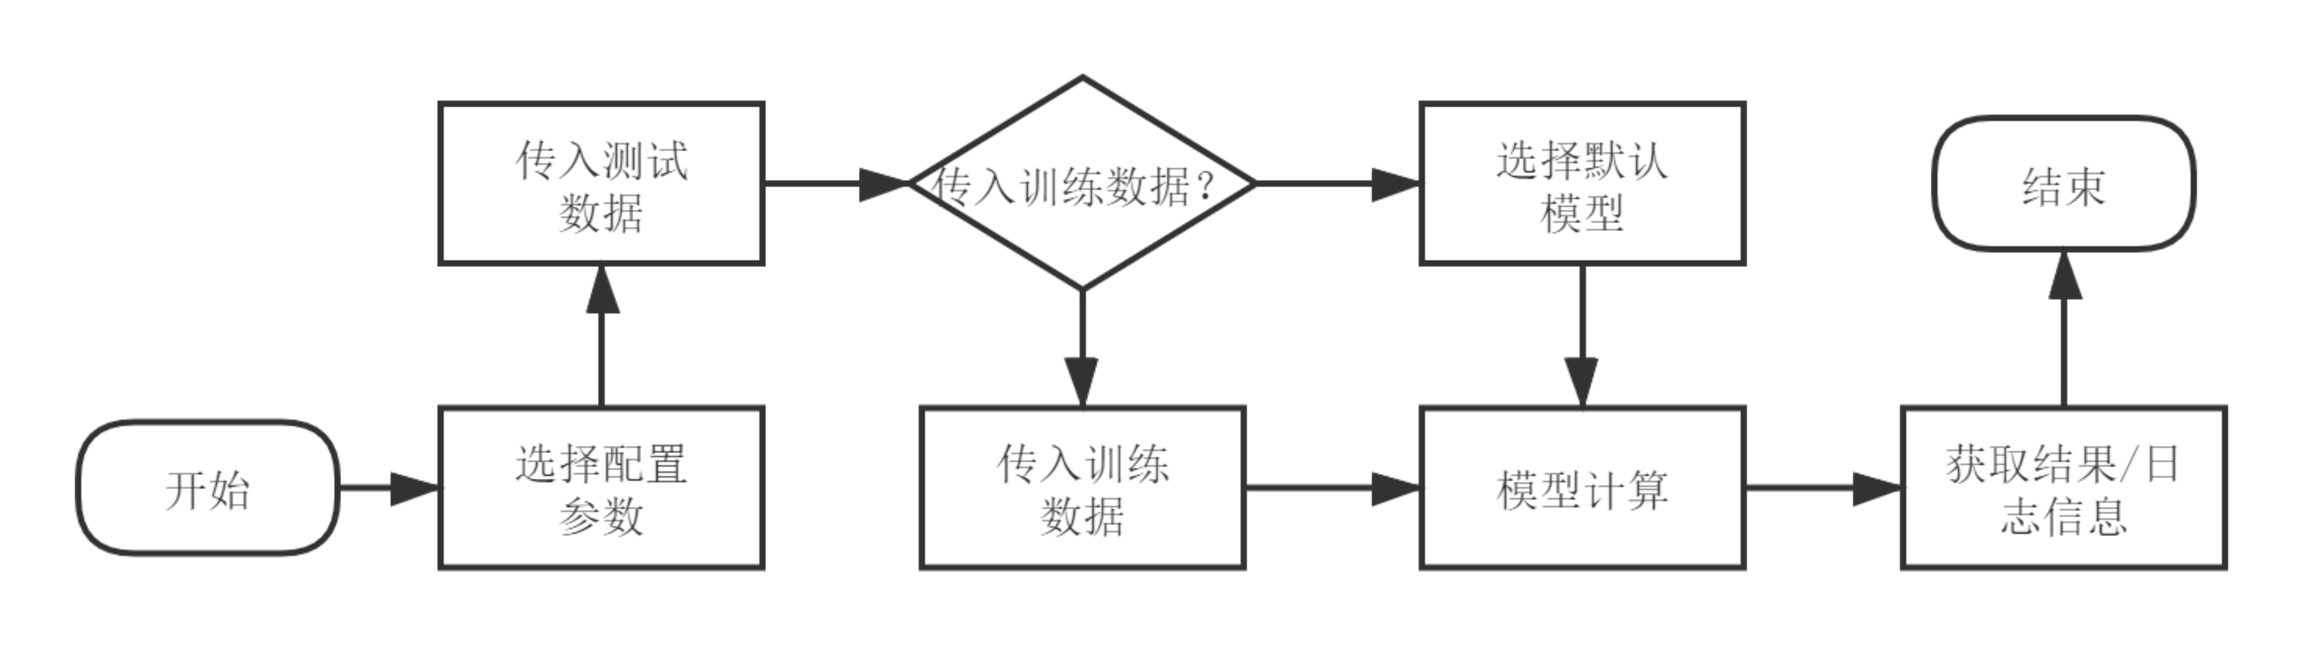
\includegraphics[width=1\textwidth]{web_pipeline.pdf}
    \caption{Metis下中文时间表达式信息抽取系统工作流程}
    \label{fig:web_pipeline}
\end{figure}

因此,metis 可以采取模块化的方式进行配置,即模块调用需要配置数据传输方式以及调用模块的方式,之后按照上线打包的方式就可以在 web 端使用。

通过模块化的设计,将整个用户需求分成一系列步骤来处理,在每一步中都只用考虑对应的任务,这种模块化的方法将开发和应用分开,不仅可以方
便的进行模型开发,应用时只需要额外定义一个调用方法,便很简单方便地完成配置。其次,将任务以模块划分,将系统的功能相独立,可以实现系统的高拓展
性及可维护性。

Metis 中,包括输入模块、输出模块在内的所有流程都是模块化的,每个模块都有对应的 inputs、outputs 和 options。文档分类模块旨在判断文档类型属于电子版或图片版,判断逻辑影响输出 outputs,
不同的输出会分别作为 PDF 页面分割模块和 OCR 识别模块的输入 inputs,而PDF 分割页面模块中的循环逻辑则由模块内 options 决定。整个流程是线性执行的,而每个模块的输出都可以连接到结果展示模块,以方便用户预览和下载数据。

将若干测试数据输入对应的UI测试页面,可以得到相应的结果,其结果如图~\ref{fig:web_result}所示。 其中OPERATORROOT即为上文中提到的操纵符作为根节点识别到的结果,TIMEROOT则是文本作为准确的时间刻度识别到的文本。


\begin{figure}[h]
    \centering
    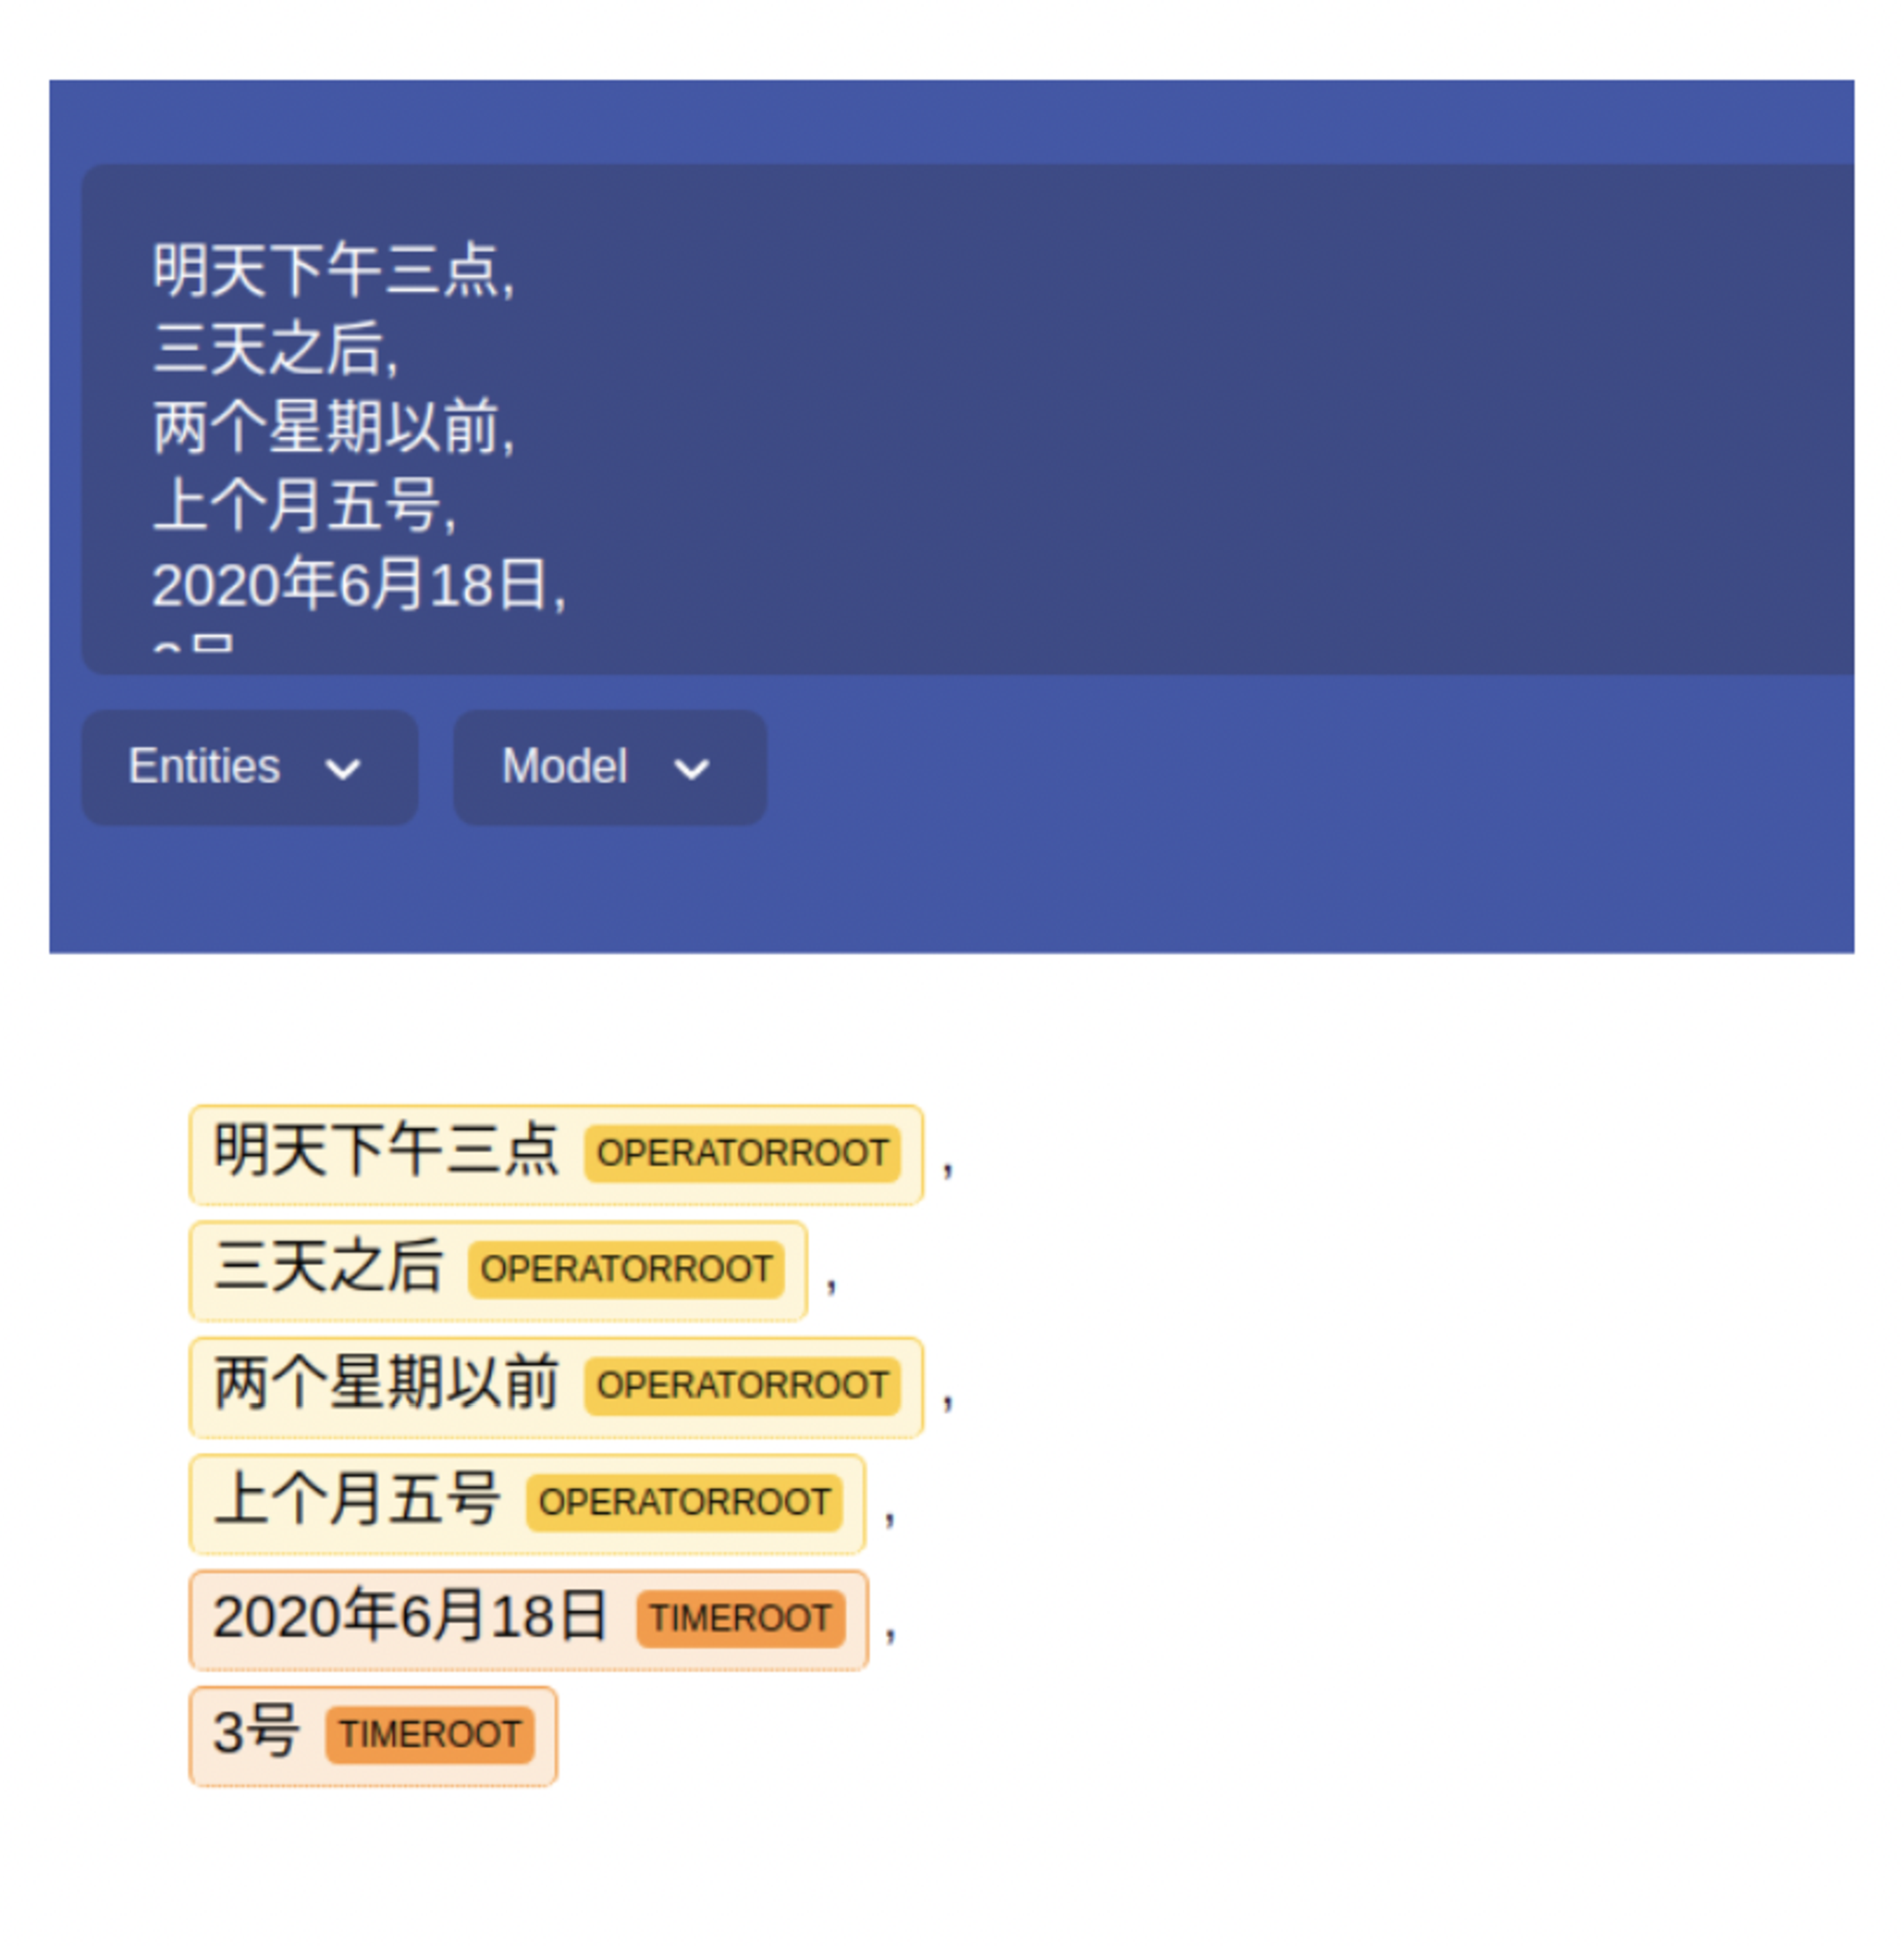
\includegraphics[width=0.75\textwidth]{web_result.pdf}
    \caption{UI测试页面}
    \label{fig:web_result}
\end{figure}


\section{时间信息抽取系统分析结果与语料存取模块}


时间信息抽取系统分析结果与语料存取模块主要是将用户传入的数据以及解析后的结果记录在MongoDB中,用户传入的数据首先会在内存中转换为Json形式,再通过序列化的方式传入MongoDB中进行持久化操作。 
当前时间信息抽取系统分析结果与语料存取模块包含将Json文件导入数据库、数据完整性校验、数据分表存储、数据表索引加速等功能。数据持久化的工作流程如图所示。


\begin{figure}[h]
    \centering
    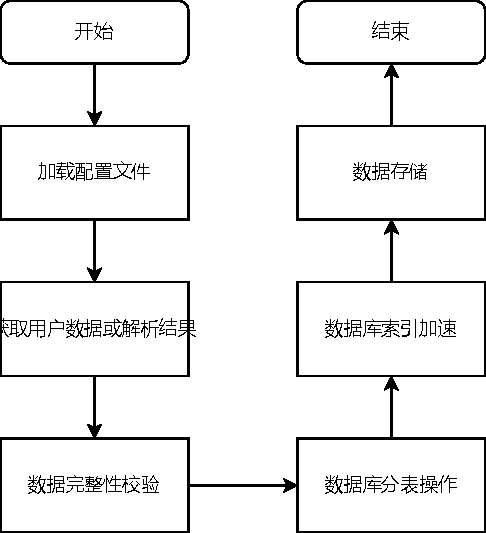
\includegraphics[width=0.5\textwidth]{database.pdf}
    \caption{存取模块工作流程}
    \label{fig:database}
\end{figure}



\section{本章小结}

本章主要介绍了基于概率无关上下文语法的中文时间表达式信息抽取系统的详细设计和实现,
首先从整体描述了系统的架构和各个模块的结构,包括中文时间表达式识别模块的设计与实现、中文时间表达式识别模块的设计与实现、
时间信息抽取系统分析与展示模块的设计与实现、时间信息抽取系统分析结果与预料存储模块的设计与实现。
部分模块还给出了相关流程图和类图详细设计。
